\subsection{Aeronautics \& Quaternions}
Aeronautics often deal with the problem of rotation.
An airplane has an ``internial frame", which needs to be corresponded to the `` body frame."
A common way to represent rotation on an airplane is with the following convention:
\begin{figure}[H]
\centering
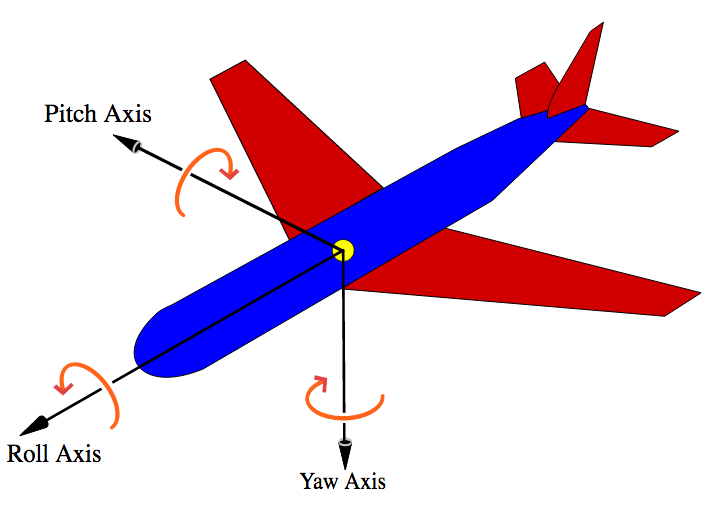
\includegraphics[width = .75\textwidth]{Figures/plane.png}
\caption{Roll, Pitch, and Yaw}
\label{fig:cycle}
\end{figure}
Roll, pitch, and yaw are simply Euler angles.
When flying a small plane, and rotating about a single axis, it may be easier to use Euler angles.
However, many large commerical airlines use computer assisted flight with many maneuvers done on autopilot.
Complicated rotations may be represented as an arbitrary rotation about an arbitrary axis, the perfect use case for quaternions.
There is another reason to use quaternions rather than rotation matrices when flying.
Rotations in 3D space can be thought of as a three gimbal system, where a gimbal is `` a pivoted support that allows the rotation of an object about a single axis.''
Figure \ref{fig:gimbal} shows an example of a 3-axis gimbal system.
\begin{figure}[H]
\centering
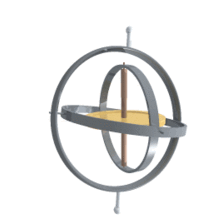
\includegraphics[width = .75\textwidth]{Figures/gimbal.png}
\caption{A 3-Axis Gimbal System}
\label{fig:gimbal}
\end{figure}
 This is essentially a visualization of Euler angles, where the deviation from the traditional 3-axis orientation can be used to keep track of the orientation of the system.
 Gimbals are commonly used in gyroscopes, aeronautics, and rocket systems.
 Gimbals in a 3-axis configuration have 3 degrees of freedom.
 A phenomenon can occur where gimbals end up in the same plane, and you lose a degree of freedom.
 Figure \ref{fig:gimlock} shows a locked gimbal system.

 \begin{figure}[H]
 \centering
 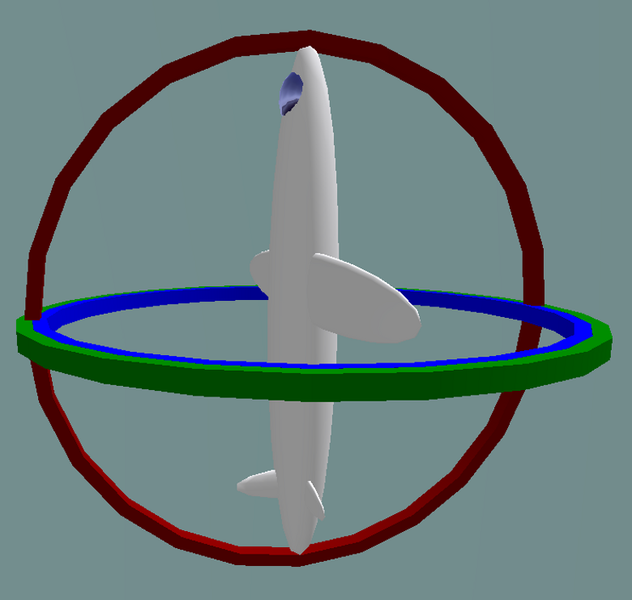
\includegraphics[width = .75\textwidth]{Figures/gimbal_lock.png}
 \caption{Roll and Yaw Gimbal Locked System}
 \label{fig:gimlock}
 \end{figure}

 In the above figure, the roll and yaw axes are now represented with a single gimbal.
 If the plane is told to rotate roll or yaw, the rotation is applied to the same axis.
 The only way to get out of gimbal lock is to rotate about the single gimbal.
 Gimbal lock is a property of Euler angles and rotation matrices.
 Recall the rotation matrix R that we calculated for ($\phi, \theta, \psi$).
 
 $$
 R =
 \begin{bmatrix}
 \text{cos }\psi \text{ cos }\phi- \text{cos }\theta \text{ sin }\phi \text{ sin }\psi & \text{cos } \psi \text{ sin }\theta + \text{cos }\theta \text{ cos }\phi \text{ sin }\psi & \text{sin }\psi \text{ sin }\theta \\
 -\text{sin }\psi \text{ cos }\phi - \text{cos }\theta \text{ sin }\phi \text{ cos }\psi & - \text{sin }\psi \text{ sin }\phi + \text{cos }\theta \text{ cos }\phi \text{ sin }\psi & \text{cos }\psi \text{ sin }\theta \\
 \text{sin }\theta \text{ sin }\phi & - \text{sin }\theta \text{ cos }\theta & \text{cos } \theta
 \end{bmatrix}
 $$



\subsection{Computer Graphics \& Quaternions}
